\documentclass{beamer}
\usepackage{tikz}
\usetikzlibrary{calc}
\usepackage{xcolor}

\title{Fractions: Starters}
\author{}
\date{}

\begin{document}

\frame{\titlepage}

%------------------------------------------------
% SLIDE 1: Equal Sharing and Part-Whole (Merged)
%------------------------------------------------
\begin{frame}{Starter 1}

\begin{columns}
\column{0.45\textwidth}
\begin{center}
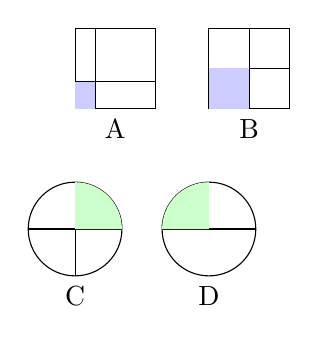
\begin{tikzpicture}[scale=0.85]
% A: Unequal
\draw (0,0) rectangle (1.2,1.2);
\draw (0,0.4) -- (1.2,0.4);
\draw (0.3,0) -- (0.3,1.2);
\fill[blue!20] (0,0) rectangle (0.3,0.4);
\node at (0.6,-0.3) {A};
% B: Equal
\draw (2,0) rectangle (3.2,1.2);
\draw (2,0.6) -- (3.2,0.6);
\draw (2.6,0) -- (2.6,1.2);
\fill[blue!20] (2,0) rectangle (2.6,0.6);
\node at (2.6,-0.3) {B};
% C: Equal
\draw (0,-1.8) circle (0.7);
\draw (0,-1.8) -- (0.7,-1.8);
\draw (0,-1.8) -- (-0.7,-1.8);
\draw (0,-1.8) -- (0,-1.1);
\draw (0,-1.8) -- (0,-2.5);
\fill[green!20] (0,-1.8) -- (0.7,-1.8) arc (0:90:0.7) -- cycle;
\node at (0,-2.8) {C};
% D: Unequal
\draw (2,-1.8) circle (0.7);
\draw (2,-1.8) -- (2.7,-1.8);
\draw (2,-1.8) -- (2,-1.1);
\draw (2,-1.8) -- (1.3,-1.8);
\fill[green!20] (2,-1.8) -- (2,-1.1) arc (90:180:0.7) -- cycle;
\node at (2,-2.8) {D};
\end{tikzpicture}
\end{center}

\column{0.55\textwidth}
\textbf{Questions}
\begin{enumerate}
    \item Which shapes (A, B, C, D) are divided into equal parts?
    \item In shape B, what fraction is shaded? 
    \item Draw a rectangle divided into 5 equal parts. Shade $\frac{3}
    {5}$.
    \item Which is larger: $\frac{2}{5}$ or $\frac{3}{5}$?
    \item Which is larger: $\frac{3}{5}$ or $\frac{3}{4}$?
    \item Order the following fractions from smallest to largest: \newline $\frac{1}{100}, \frac{100}{1}, \frac{1}{10}, \frac{10}{1}, \frac{1}{1}$
\end{enumerate}
\end{columns}

\end{frame}

%------------------------------------------------
% SLIDE 2: Equivalent Fractions
%------------------------------------------------
\begin{frame}{Starter 2}

\begin{columns}
\column{0.45\textwidth}
\begin{center}
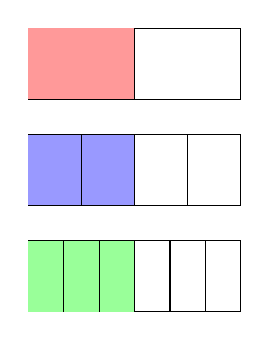
\begin{tikzpicture}[scale=0.9]
% Bar 1/2
\draw (0,0) rectangle (3,1);
\fill[red!40] (0,0) rectangle (1.5,1);

\draw (1.5,0) -- (1.5,1);
% Bar 2/4
\draw (0,-1.5) rectangle (3,-0.5);
\fill[blue!40] (0,-1.5) rectangle (1.5,-0.5);
\draw (0.75,-1.5) -- (0.75,-0.5);
\draw (1.5,-1.5) -- (1.5,-0.5);
\draw (2.25,-1.5) -- (2.25,-0.5);
% Bar 3/6
\draw (0,-3) rectangle (3,-2);
\fill[green!40] (0,-3) rectangle (1.5,-2);
\foreach \x in {0.5,1,1.5,2,2.5} {
    \draw (\x,-3) -- (\x,-2);
}

\end{tikzpicture}
\end{center}

\column{0.55\textwidth}
\textbf{Questions}
\begin{enumerate}
    \item Write the fraction shaded for each bar.
    \item Is the same proportion of each bar shaded?
    \item Use the bars to fill in the blanks: $\frac{?}{2} = \frac{?}{4} = \frac{?}{6}$
    \item Shade $\frac{2}{3}$ of a bar divided into 9 parts. 
    \item Find the missing numerator: $\frac{2}{3} = \frac{?}{9}$
    \item Find the missing numerator: $\frac{1}{3} = \frac{?}{6}$.
    \item Which two fractions are equivalent: $\frac{1}{2}, \frac{2}{5}, \frac{4}{8}, \frac{3}{6}$?
\end{enumerate}
\end{columns}

\end{frame}

%------------------------------------------------
% SLIDE 3: Comparing Fractions
%------------------------------------------------
\begin{frame}{Starter 3: Comparing Fractions}

\begin{columns}
\column{0.45\textwidth}
\begin{center}
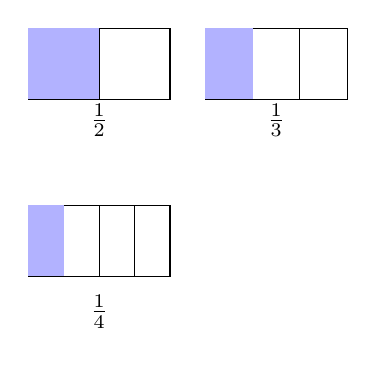
\begin{tikzpicture}[scale=0.9]
\draw (0,0) rectangle (2,1);
\draw (1,0) -- (1,1);
\fill[blue!30] (0,0) rectangle (1,1);
\node at (1,-0.3) {$\frac{1}{2}$};
\draw (2.5,0) rectangle (4.5,1);
\draw (3.17,0) -- (3.17,1);
\draw (3.83,0) -- (3.83,1);
\fill[blue!30] (2.5,0) rectangle (3.17,1);
\node at (3.5,-0.3) {$\frac{1}{3}$};
\draw (0,-2.5) rectangle (2,-1.5);
\draw (0.5,-2.5) -- (0.5,-1.5);
\draw (1,-2.5) -- (1,-1.5);
\draw (1.5,-2.5) -- (1.5,-1.5);
\fill[blue!30] (0,-2.5) rectangle (0.5,-1.5);
\node at (1,-3) {$\frac{1}{4}$};
\end{tikzpicture}
\end{center}

\column{0.55\textwidth}
\textbf{Questions}
\begin{enumerate}
    \item Which is larger: $\frac{1}{2}$ or $\frac{1}{3}$? 
    \item Compare $\frac{2}{5}$ and $\frac{4}{5}$. Which is bigger?
    \item Convert $\frac{3}{4}$ and $\frac{5}{8}$ to a common denominator. Which is larger?
    \item Order from smallest to largest: $\frac{1}{3}, \frac{1}{6}, \frac{1}{2}$.
    \item Sam ate $\frac{2}{3}$ of a pizza, Lee ate $\frac{5}{6}$ of the same pizza. Who ate more?
    \item Compare $\frac{4}{6}$ and $\frac{2}{3}$. 
\end{enumerate}
\end{columns}

\end{frame}

%------------------------------------------------
% SLIDE 4: Fractions in Real Life
%------------------------------------------------
\begin{frame}{Starter 4}

\begin{columns}
\column{0.45\textwidth}
\begin{center}
\textbf{Fractions everywhere}
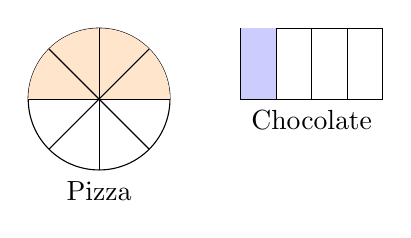
\begin{tikzpicture}[scale=0.9]
\draw (0,0) circle (1);
\fill[orange!20] (0,0) -- (0:1) arc (0:90:1) -- cycle;
\fill[orange!20] (0,0) -- (90:1) arc (90:180:1) -- cycle;
\foreach \a in {0,45,90,135,180,225,270,315} {
    \draw (0,0) -- (\a:1);
}

\node at (0,-1.3) {Pizza};
\draw (2,0) rectangle (4,1);
\draw (2.5,0) -- (2.5,1);
\draw (3,0) -- (3,1);
\draw (3.5,0) -- (3.5,1);
\fill[blue!20] (2,0) rectangle (2.5,1);
\node at (3,-0.3) {Chocolate};
\end{tikzpicture}
\end{center}

\column{0.55\textwidth}
\textbf{Questions}
\begin{enumerate}
    \item A cake is cut into 10 equal slices. If 3 are eaten, what fraction remains?
    \item There are 30 students. $\frac{2}{5}$ walk to school. How many walk?
    \item A ruler is 24 cm long. Mark $\frac{1}{2}$ and $\frac{1}{3}$ on it. How many cm is each?
    \item Which is longer: $\frac{3}{4}$ of an hour or $\frac{2}{3}$ of an hour? (1 hour = 60 mins)
    \item You have \$30. You spend $\frac{2}{5}$ on a book. How much do you spend? How much left?
    \item A recipe needs $\frac{3}{4}$ cup of milk. You only have a $\frac{1}{4}$ cup measure. How many times must you fill it?
\end{enumerate}
\end{columns}

\end{frame}

\end{document}